\documentclass[12pt, a4paper]{article}
\usepackage{fstyle}
\usepackage{enumitem}

\graphicspath{ {./img/} }
\def\arraystretch{2} %define table vertical spacing
\setlist{nolistsep,leftmargin=*} %remove list spacing
\newcolumntype{Y}{>{\centering\arraybackslash}X} %new tabularx centered X column  

\begin{document}
\title{CheatSheet di Analisi Matematica}
\author{Fabio Ferrario}
\date{2022}
\maketitle
\section*{Studio di Funzione}
Per lo studio di una funzione bisogna trovare:
\paragraph*{Dominio} della funzione, poni:\\

\begin{tabular}{ l|l }
	Denominatore    & $\leq 0$                                 \\
	Logaritmo       & Argomento $>0$                           \\
	Radice$^n$      & Argomento $\geq 0$ (\emph{sse $n$ pari}) \\
	$[f(x)]^{g(x)}$ & $f(x)>0$
\end{tabular}
\paragraph*{Limiti ai punti di frontiera del dominio}
Trovato il dominio, trova \emph{i limiti ai punti di frontiera},
quindi porre i limiti ad ogni punto in cui il dominio si interrompe (sia da destra che da sinistra) e eventualmente a $\pm \infty$.
\paragraph*{Asintoti}
Trovati tutti i limiti, se trovi:
\begin{itemize}
	\item $\limite{x}{\alpha^\pm} f(x) = \pm \infty \implies$ Asintoto \emph{Verticale}.
	\item $\limite{x}{\pm \infty} f(x) = l \implies$ Asintoto \emph{Orizzontale} (di equazione $y=l$)
\end{itemize}
Bisogna anche controllare la presenza di \textbf{Asintoti Obliqui}:
\begin{itemize}
	\item $m = \limite{x}{\pm \infty} \frac{f(x)}{x} \implies$ se $m$ \emph{esiste e non è nullo} trovo $q$:
	\item $q = \limite{x}{\pm \infty} [f(x) - mx]\implies$  se $q$ esiste allora $y=mx+q$ è \emph{asintoto obliquo}
\end{itemize}
\paragraph*{Monotonia}
La monotina di una funzione si calcola \emph{ponendo $f'(x)>0$.}
Nei punti in cui la derivata è positiva, la funzione è \textbf{Crescente}, nei punti in cui è negativa la funzione è \textbf{Decrescente}
\paragraph*{Punti di estremo}
Una volta trovato il segno della derivata si possono trovare i punti di estremo.
\\I punti in cui la derivata cambia direzione sono punti di estremo
\paragraph*{Convessità/Concavità}


\paragraph*{Retta Tangente} al grafico in $x_0$:\\
trova $y=mx + q$ ponendo:
\begin{itemize}
	\item $m=f'(x_0)$
	\item $q=f(x_0)-f'(x_0)\cdot x_0$
\end{itemize}


\section*{Serie}
\subsection*{Serie Notevoli}
\paragraph*{Serie Armonica Generalizzata}
\begin{equation*}
	\sum \frac{1}{n^\alpha} \begin{cases}
		\text{Diverge}  & \alpha\leq 1 \\
		\text{Converge} & \alpha> 1
	\end{cases}
\end{equation*}
\paragraph*{Serie Geometrica}
\begin{equation*}
	\serie{0}{+\infty} q^n \begin{cases}
		\text{Diverge}    & q\geq 1 \\
		\text{Converge}   & -1<q<1  \\
		\text{Irregolare} & q\leq 1
	\end{cases}
\end{equation*}
\subsection*{Criteri di Convergenza}

\emph{Condizione necessaria ma non sufficiente} di convergenza è che il termene generale $a_n$ sia infinitesimo $\limite{n}{+\infty} a_n = 0$.
\\Avendo $a_n>0$ (positiva) \emph{definitivamente} posso usare i seguenti criteri:
\begin{itemize}
	\item \textbf{Rapporto}: $\limite{n}{+\infty} \frac{a_n+1}{a_n} = l$
	\item \textbf{Radice}: $\limite{n}{+\infty} \sqrt[n]{a_n} = l$
\end{itemize}
In entrambi questi casi $\sum a_n$:\\
\emph{Converge} se $l<1$, \emph{Diverge} se $l>1$ e il criterio è \emph{inconclusivo} se $l=1$

\begin{itemize}
	\item \textbf{Confronto}: $a_n\leq b_n$ definitivamente $\implies$
	      \begin{itemize}
		      \item se $b_n$ converge, allora $a_n$ converge.
		      \item se $a_n$ diverge positivamente, allora anche $b_n$
	      \end{itemize}
\end{itemize}

\paragraph*{Criterio dell'Assoluta Convergenza}
$\sum a_n$ Converge assolutamente se converge $\sum |a_n|$.
Se una serie converge assolutamente, allora converge.

\section*{Limiti}

	\paragraph*{\underline{Limiti Notevoli}}

	\begin{tabularx}{0.8\textwidth}{ |X|X| }
		\hline
		Logaritmo naturale          & $\limite{x}{0} \frac{\ln(1+x)}{x} = 1 $  \\
		\hline
		Logaritmo con base $a$          & $\limite{x}{0} \frac{\log_a(1+x)}{x} = \frac{1}{\ln(a)} $  \\
		\hline
		$f$ Esponenziale    & $\limite{x}{0} \frac{e^x-1}{x} = 1$      \\
		\hline
		$f$ Esponenziale base $a$    & $\limite{x}{0} \frac{a^x-1}{x} = \ln(a)$      \\
		\hline
		Costante e Frazione & $\limite{x}{0}\frac{ax -1}{x} = \ln(a)$  \\
		\hline
		Seno                & $\limite{x}{0}\frac{\sin(x)}{x} = 1$     \\
		\hline
		Coseno              & $\limite{x}{0} \frac{1-\cos(x)}{x} = 0 $ \\
		\hline
	\end{tabularx}


	\paragraph*{\underline{Equivalenze Asintotiche}}

	\begin{tabularx}{0.67\textwidth}{|XYX|}
		\hline
		\multicolumn{3}{|c|}{\textbf{con \emph{x} $\to$ 0}} \\
		\hline
		\hline
		$\sin x$           & $\sim$ & $x$                   \\
		\hline
		$1-\cos x$         & $\sim$ & $\frac{1}{2}x^2$      \\
		\hline
		$\tan x$           & $\sim$ & $x$                   \\
		\hline
		$\ln(1+x)$         & $\sim$ & $x$                   \\
		\hline
		$(1+x)^\alpha -1 $ & $\sim$ & $\alpha x$            \\
		\hline
	\end{tabularx}

\begin{multicols}{2}
	\paragraph*{\underline{Ordine degli infiniti}}$\infty$
	\columnbreak
	$$ \log_ax\ll x^b\ll x^c\ll d^x\ll g^x\ll x^x $$
\end{multicols}
\begin{center}
	\small{NB: la radice è "più grande" del logaritmo}
\end{center}

\paragraph*{\underline{Forme di indecisione}}.\\
\begin{tabularx}{\textwidth}{|l|X|}
	\hline
	\multicolumn{2}{|c|}{
		$[\frac{0}{0}]$ $[\frac{\infty}{\infty}]$ $[1^\infty]$ $[\infty - \infty]$ $[\infty \cdot 0]$ $[0^0]$ $[\infty^0]$
	}                                                                                         \\
	\hline
	\multicolumn{2}{|X|}{
		\small{Tutte le forme possono essere risolte usando \textbf{Limiti Notevoli} e \textbf{Trucchi algebrici} per ricondursi ad essi.
			In particolare però, questi si risolvono usando anche:}
	}                                                                                         \\
	\hline
	$[\frac{0}{0}]$           & Conf. infinitesmi | Scomp/Racc/Semp | De l'Hopital            \\
	\hline
	$[\frac{\infty}{\infty}]$ & Conf. infinti | Scomp/Racc/Semp | De l'Hopital                \\
	\hline
	$[1^\infty]$              & Identità Logaritmo-Esponenziale                               \\
	\hline
	$[\infty - \infty]$       & Riconduzione a $\frac{0}{0}$ o $\frac{\infty}{\infty}$        \\
	\hline
	$[\infty \cdot 0]$        & Razionalizzazione inversa | Prodotti notevoli al contrario    \\
	\hline
	$[0^0]$ / $[\infty^0]$    & Conf. infiniti/infinitesimi|Identità Logaritmo-Esponenziale \\
	\hline
\end{tabularx}


\section*{Calcolo Differenziale}

\paragraph*{\underline{Derivata dell'inversa di una funzione}}
Dati:\\
$y_o$ e $f(x)$, avendo $g(x) = f^{-1}(x)$ allora:
Per calcolare $g'(y_0)$
\begin{enumerate}
	\item trovo $x_0$ ponendo $y_0=f(x)$
	\item trovo $g'(y_0)=\frac{1}{f'(x_0)}$
\end{enumerate}

\paragraph*{\underline{Formula di Taylor}} di grado $k$ e centrato in $x_0$:
$$P_k(x)=f(x_0)+f'(x_0)(x-x_0) + \frac{1}{2}f''(x_0)(x-x_0)^2 +... + \frac{1}{k!}f^{(k)}(x_0)(x-x_0)^k$$

\paragraph*{\underline{Formula di Mclaurin}} di grado $k$:
$$P_k(x)=f(0)+f'(0)x+\frac{1}{2}f''(0)x^2+...+\frac{1}{k!}f^{(k)}(0)x^k$$
\small{Mclaurin = Taylor con $x_0=0$}

\paragraph*{\underline{Rapporto incrementale}}
$$\frac{\Delta y}{ \Delta x}\frac{f(x_0+h)-f(x_0)}{h} $$


\section*{Calcolo Integrale}

\begin{multicols}{3}
\paragraph*{\underline{Primitive elementari}}
Funzioni il cui integrale è immediatamente calcolabile.
\columnbreak
\begin{tabularx}{0.7\textwidth}{ |Y|Y| }
	\hline
	\textbf{Funzione} & \textbf{Primitiva}    \\
	\hline
	$k$               & $kx$                  \\
	$x^a$,$a\neq-1$   & $\frac{x^{a+1}}{a+1}$ \\
	$\frac{1}{x}$     & $\log|x|$             \\
	$\sin x$          & $-\cos x$             \\
	$\cos x $         & $\sin x$              \\
	$a^x$             & $\frac{a^x}{\log a}$  \\
	\hline
	$e^{-x}$          & $-e^{-x}$             \\
	\hline
\end{tabularx}
\end{multicols}

\paragraph*{Proprietà degli integrali}
\begin{itemize}
	\item Somma di integrali: $\int f(x)+g(x) dx = \int f(x) dx + \int g(x) dx$
	\item Costante moltiplicativa $\int k \cdot f(x) = k \int f(x)$
\end{itemize}
\subsection*{I metodi di risoluzione}
\paragraph*{Integrazione per Parti}
$$\int f(x)g'(x)dx = f(x)g(x)-\int f'(x)g(x)dx$$
\begin{center}
	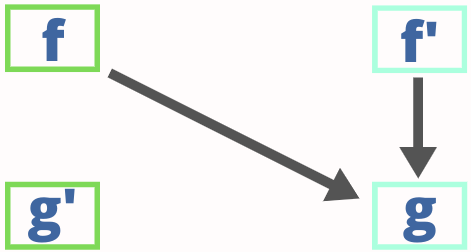
\includegraphics[width=0.4\textwidth]{integrazione-per-parti.png}
\end{center}

\paragraph*{\underline{Integrazione per Sostituzione}} 
\subparagraph*{\emph{Metodo Generale e Semplificato}} per itnegrali generali $f(x)$:
\\Trovo una funzione $g(x)$ \emph{Derivabile e Invertibile} da sostituire ad $x$.
\begin{enumerate}
	\item decido che $y=g(x)$
	\item Inverto $g(x)$ per isolare la x, ottenendo $x=g^{-1}(y)$
	\item Derivo entrambi i membri e aggiungo $dx$ e $dy$: $\to dx=(g^{-1})'(y)dy$
	\item all'interno di $f(x)$ sosdtituisco $g(x) \to y$ e $dx \to (g^{-1})'(y)dy$
	\item Risolvo l'integrale
	\item Sostiuisco $y \to g(x)$ 
\end{enumerate}
\subparagraph*{Metodo dalla definizione}: Abbiamo un integrale nella forma
$$\int f((g(x))g'(x) dx$$
\begin{enumerate}
	\item $y=g(x)\to dy=g'(y)dx$
	\item Sostituiamo per ottenere $\int f(y)dy$
	\item Calcolo l'integrale nella nuova variabile
	\item Sostituisco $y\to g(x)$
\end{enumerate}




\end{document}